% Provenance (never printed): cycle 2 "Questionner l'espace et le temps ---
% se situer dans l'espace": representations of familiar spaces (plans), "lire
% des plans, se reperer sur des cartes. Elements constitutifs d'une carte :
% titre, echelle, orientation, legende"; see sources/book1/PROVENANCE.md.
% Book 1, grade 2, chapter 2. Sync 1: "scale" is owned here; "cardinal
% directions" is the physics series' term (prose only); "compass rose" here.
\chapter{Du dessin à la carte}\label{ch:g2:drawing-to-map}

Un pigeon survole l'école. Que voit-il~? Ni les portes d'entrée, ni les
fenêtres, ni le visage des enfants~: de là-haut, il ne voit que le dessus
des choses. Les toits des bâtiments sont des rectangles gris. La cour est
une grande forme vide avec quelques cimes d'arbres toutes rondes. Les
allées sont des traits fins. Le pigeon voit l'école d'en haut --- comme la
montre une \omterm{def:g2:drawing-to-map:map}{carte}.

\begin{omfigure}
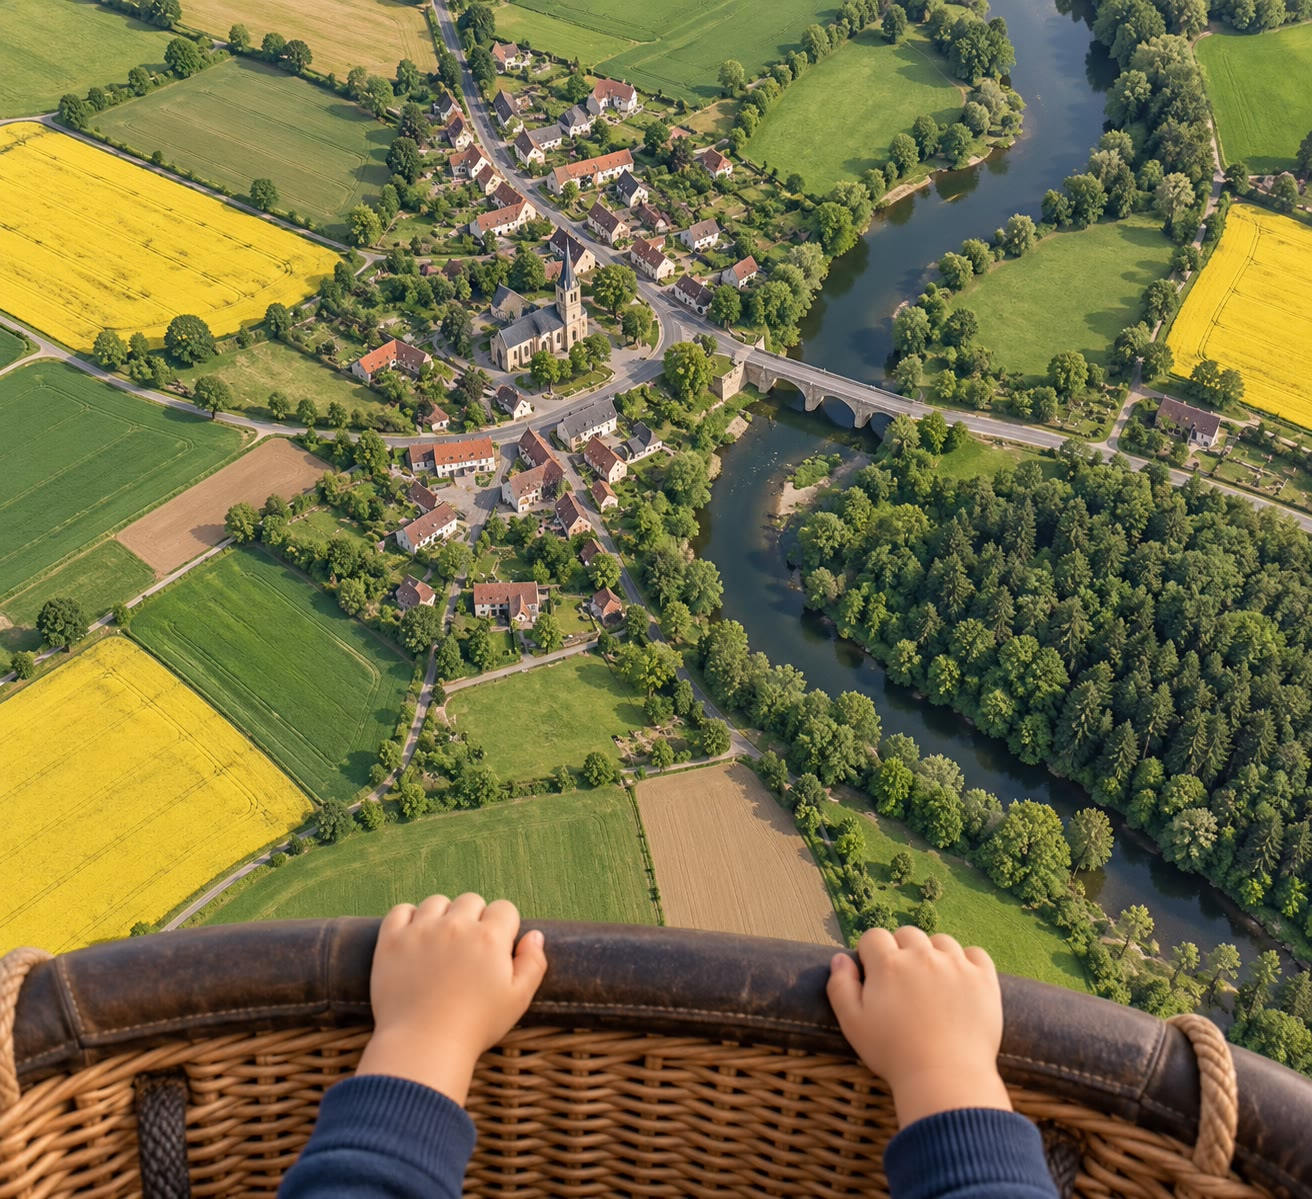
\includegraphics[width=0.62\linewidth]{images/book1/ai/g2-balloon-view.jpg}

{\small La campagne vue d'une montgolfière~: des champs, un village, une
route, une \omterm{def:g1:landscapes-around-us:water}{rivière} et son pont, le tout vu d'en haut.}
\end{omfigure}

\section{Vu de côté, vu d'en haut}

Pose quelques cubes de jeu sur une table. Regarde-les de côté~: tu vois
leur hauteur, et ceux de derrière sont cachés par ceux de devant.
Maintenant, lève-toi et regarde-les d'en haut~: tu ne vois plus leur
hauteur, mais tu vois exactement où est chacun d'eux, et à quelle
distance ils sont les uns des autres.

\begin{omfigure}
\begin{tikzpicture}[x=1cm, y=1cm, font=\small]
  % side view
  \begin{scope}
    \draw[black!50] (-0.2,0) -- (4.6,0);
    \fill[red!55, draw=black!60] (0.2,0) rectangle (1.2,1.6);
    \fill[ocBlue!55, draw=black!60] (1.6,0) rectangle (3.0,0.8);
    \fill[yellow!70, draw=black!60] (3.4,0) -- (3.9,1.1) -- (4.4,0) -- cycle;
    \node at (2.2,-0.5) {vu de côté};
  \end{scope}
  % from above
  \begin{scope}[shift={(6.4,0)}]
    \draw[black!30, fill=black!3] (-0.2,-0.1) rectangle (4.6,2.3);
    \fill[red!55, draw=black!60] (0.2,0.4) rectangle (1.2,1.4);
    \fill[ocBlue!55, draw=black!60] (1.6,1.0) rectangle (3.0,2.0);
    \fill[yellow!70, draw=black!60] (3.9,0.75) circle (0.5);
    \node at (2.2,-0.5) {vu d'en haut};
  \end{scope}
\end{tikzpicture}

{\small Trois cubes sur une table~: un grand cube rouge, un cube bleu tout
plat et un cône jaune. Vu d'en haut, le cône est un disque et le grand
cube est un carré.}
\label{fig:g2:drawing-to-map:blocks}
\end{omfigure}

\begin{definition}[Plan]\label{def:g2:drawing-to-map:plan}
Un \emph{plan}\index{plan} est le dessin d'un petit lieu --- une pièce,
une maison, une école, un jardin --- tel qu'on le voit exactement d'en
haut, dessiné plus petit qu'en vrai, mais avec chaque partie à sa place.
\end{definition}

\section{Dessiner plus petit~: l'échelle}

Une salle de classe est bien trop grande pour être dessinée telle quelle
sur une feuille de papier. Nous la dessinons plus petite --- mais chaque
partie doit être réduite de la même façon, sinon le \omterm{def:g2:drawing-to-map:plan}{plan} ment. Le plus
simple est d'utiliser du papier quadrillé~: un carreau du papier
représente un mètre de la classe.

\begin{definition}[Échelle]\label{def:g2:drawing-to-map:scale}
L'\emph{échelle}\index{echelle@échelle} d'un \omterm{def:g2:drawing-to-map:plan}{plan} ou d'une \omterm{def:g2:drawing-to-map:map}{carte} dit
combien le dessin est plus petit que le lieu réel~: quelle distance sur le
terrain représente une longueur sur le dessin. Par exemple~:
\emph{1 carreau représente 1 mètre}.
\end{definition}

\begin{omfigure}
\begin{tikzpicture}[x=0.75cm, y=0.75cm, font=\scriptsize]
  \draw[black!15] (0,0) grid (10,8);
  \draw[black, line width=1.6pt] (0,0) rectangle (10,8);
  % board on the north wall
  \fill[black!70] (3,7.8) rectangle (7,8);
  % teacher's desk
  \fill[brown!50, draw=black!70] (4,6) rectangle (6,7);
  % pupils' desks: 3 rows of 3
  \foreach \x in {1,4,7} \foreach \y in {1,2.5,4}
    \fill[orange!45, draw=black!70] (\x,\y) rectangle ++(2,1);
  % cupboard
  \fill[ocBlue!40, draw=black!70] (9,5) rectangle (10,8);
  % door (gap) on the east wall, windows on the west wall
  \fill[white] (9.85,1) rectangle (10.15,2);
  \draw[black!70] (10,2) arc[start angle=90, end angle=180, radius=1];
  \foreach \y in {1.5,4.5}
    \draw[ocBlue, line width=2.5pt] (0,\y) -- (0,\y+2);
  % legend
  \begin{scope}[shift={(11,7.2)}]
    \node[anchor=west, font=\small\bfseries] at (0,0.4) {La salle de classe};
    \fill[black!70] (0,-0.25) rectangle (0.8,-0.05); \node[anchor=west] at (1,-0.15) {tableau};
    \fill[brown!50, draw=black!70] (0,-1.1) rectangle (0.8,-0.7); \node[anchor=west] at (1,-0.9) {bureau du maître};
    \fill[orange!45, draw=black!70] (0,-1.85) rectangle (0.8,-1.45); \node[anchor=west] at (1,-1.65) {table d'élève};
    \fill[ocBlue!40, draw=black!70] (0,-2.6) rectangle (0.8,-2.2); \node[anchor=west] at (1,-2.4) {placard};
    \draw[ocBlue, line width=2.5pt] (0,-3.15) -- (0.8,-3.15); \node[anchor=west] at (1,-3.15) {fenêtre};
    \draw[black!70] (0.8,-3.95) arc[start angle=0, end angle=90, radius=0.6]; \draw[black, line width=1.6pt] (0.2,-3.95) -- (0.8,-3.95); \node[anchor=west] at (1,-3.7) {porte};
    \draw[black!15] (0,-4.9) rectangle (0.75,-4.15);
    \node[anchor=west] at (1,-4.53) {1 carreau = 1 mètre};
    \pic[scale=0.7, transform shape] at (0.7,-6.2) {compassrose};
  \end{scope}
\end{tikzpicture}

{\small Le \omterm{def:g2:drawing-to-map:plan}{plan} d'une salle de classe sur papier quadrillé, avec son titre,
sa \omterm{def:g2:drawing-to-map:legend}{légende}, son \omterm{def:g2:drawing-to-map:scale}{échelle} et sa \omterm{def:g2:drawing-to-map:directions}{rose des vents}. Le mur nord, celui du
tableau, est en haut.}
\label{fig:g2:drawing-to-map:classroom}
\end{omfigure}
% (exercise data: an invented classroom of 10 m by 8 m)

\begin{method}[Mesurer sur un plan]\label{met:g2:drawing-to-map:measure}
Pour trouver une longueur réelle sur un \omterm{def:g2:drawing-to-map:plan}{plan} dessiné sur des carreaux~:
\begin{enumerate}
  \item compte les carreaux le long de la longueur que tu cherches~;
  \item lis l'\omterm{def:g2:drawing-to-map:scale}{échelle}~: ce que représente un carreau~;
  \item donne la réponse en mètres (ou en kilomètres sur une \omterm{def:g2:drawing-to-map:map}{carte}).
\end{enumerate}
\end{method}

\begin{example}[Quelle est la longueur de la classe~?]\label{ex:g2:drawing-to-map:length}
Le long du mur nord du \omterm{def:g2:drawing-to-map:plan}{plan}, il y a 10 carreaux. Un carreau représente
1 mètre, donc la classe mesure 10 mètres de long. Le long du mur ouest, il
y a 8 carreaux~: elle mesure 8 mètres de large. Le tableau occupe
4 carreaux du mur nord~: il mesure 4 mètres de long.
\end{example}

\begin{omfigure}
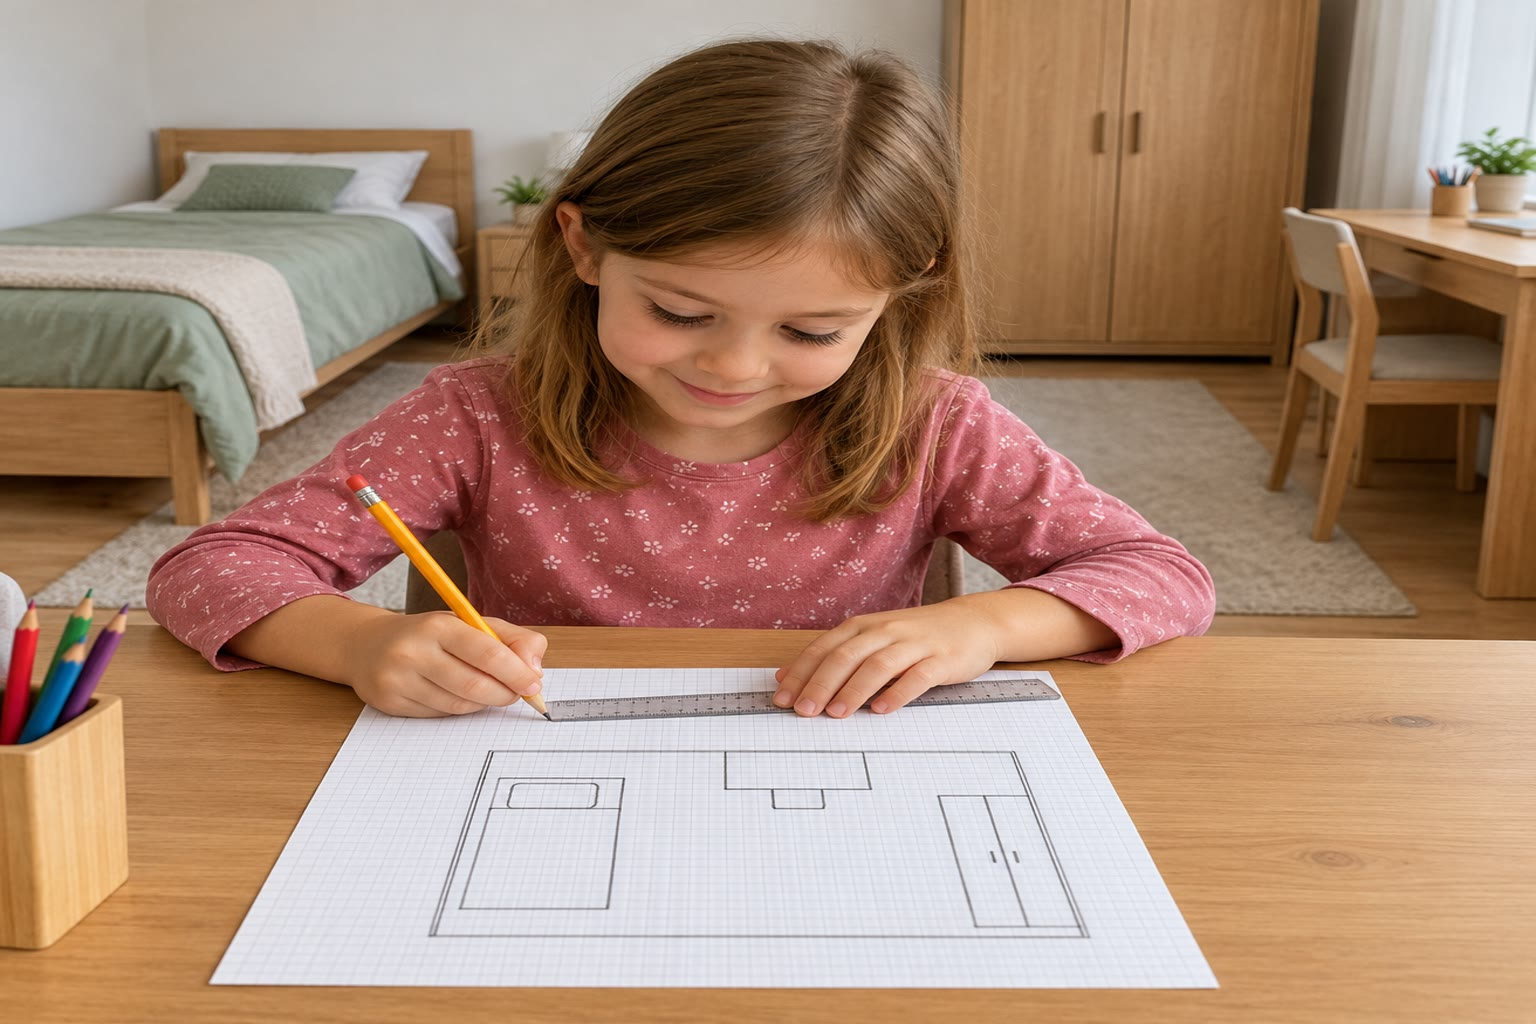
\includegraphics[width=0.55\linewidth]{images/book1/ai/g2-bedroom-plan.jpg}

{\small On dessine le \omterm{def:g2:drawing-to-map:plan}{plan} d'une chambre sur du papier quadrillé.}
\end{omfigure}

\section{Du plan à la carte}

Un \omterm{def:g2:drawing-to-map:plan}{plan} montre un petit lieu. Quand nous dessinons un lieu plus grand ---
toute une ville, une \omterm{def:g1:landscapes-around-us:landform}{vallée}, un pays ---, nous dessinons une \omterm{def:g2:drawing-to-map:map}{carte}.

\begin{definition}[Carte]\label{def:g2:drawing-to-map:map}
Une \emph{carte}\index{carte} est le dessin d'une grande partie de la
surface de la Terre, vue d'en haut et dessinée beaucoup plus petite
qu'en vrai.
\end{definition}

Sur une \omterm{def:g2:drawing-to-map:map}{carte}, une maison est bien trop petite pour être dessinée telle
qu'elle est~; les cartographes utilisent donc de petits signes~: un point
pour une ferme, un trait bleu pour une \omterm{def:g1:landscapes-around-us:water}{rivière}, une tache verte pour un
bois. Le sens de chaque signe est donné dans un cadre à côté de la \omterm{def:g2:drawing-to-map:map}{carte}.

\begin{definition}[Légende]\label{def:g2:drawing-to-map:legend}
Un \emph{symbole}\index{symbole} est un petit signe qui représente une
sorte de chose sur un \omterm{def:g2:drawing-to-map:plan}{plan} ou sur une \omterm{def:g2:drawing-to-map:map}{carte}. La \emph{légende}\index{legende@légende}
est le cadre qui montre chaque symbole de la \omterm{def:g2:drawing-to-map:map}{carte} avec son sens.
\end{definition}

\section{S'orienter~: les quatre points cardinaux et la rose des vents}

Pour dire où se trouve quelque chose, «~à gauche~» ou «~à droite~» ne
suffit pas~: ce qui est à ta gauche est à la droite de quelqu'un qui te
fait face. On utilise quatre directions qui sont les mêmes pour tout le
monde~: le nord, l'est, le sud et l'ouest. Tu les as rencontrées dans les
livres de physique, avec la boussole. Le matin, le Soleil se lève à l'est,
et le soir, il se couche à l'ouest~; le nord et le sud sont à mi-chemin
entre les deux, l'un en face de l'autre.

\begin{omfigure}
\begin{tikzpicture}[font=\small]
  \pic[scale=1.5, transform shape] at (0,0) {compassrose};
  \node[align=left, anchor=west, font=\small] at (2.6,0.3)
    {N = nord (en haut de la plupart des cartes)\\E = est (à droite)\\S = sud (en bas)\\O = ouest (à gauche)};
\end{tikzpicture}

{\small Une \omterm{def:g2:drawing-to-map:directions}{rose des vents}. Entre le nord et l'est se trouve le nord-est~;
entre le sud et l'ouest, le sud-ouest.}
\label{fig:g2:drawing-to-map:rose}
\end{omfigure}

\begin{definition}[Rose des vents]\label{def:g2:drawing-to-map:directions}
Une \emph{rose des vents}\index{rose des vents} est l'étoile dessinée sur
une \omterm{def:g2:drawing-to-map:map}{carte} qui montre les directions du nord, de l'est, du sud et de
l'ouest. Sur la plupart des \omterm{def:g2:drawing-to-map:map}{cartes}, le nord est en haut, l'est à droite,
le sud en bas et l'ouest à gauche.
\end{definition}

\begin{safety}
Ne regarde jamais le Soleil pour trouver l'est ou l'ouest~: tes yeux
pourraient être abîmés pour toujours. Regarde plutôt les ombres, ou
sers-toi d'une boussole.
\end{safety}

\section{Lire une vraie carte}

Toute bonne \omterm{def:g2:drawing-to-map:map}{carte} a quatre éléments~: un \textbf{titre} qui dit ce que
montre la \omterm{def:g2:drawing-to-map:map}{carte}, une \textbf{\omterm{def:g2:drawing-to-map:legend}{légende}}, une \textbf{\omterm{def:g2:drawing-to-map:scale}{échelle}} et une
\textbf{\omterm{def:g2:drawing-to-map:directions}{rose des vents}} (ou au moins une flèche qui indique le nord).
Voici la \omterm{def:g2:drawing-to-map:map}{carte} d'une \omterm{def:g1:landscapes-around-us:landform}{vallée} vallonnée, les collines de Varden. C'est la
\omterm{def:g1:landscapes-around-us:landform}{vallée} inventée que tu retrouveras encore et encore dans ce livre et dans
les suivants, chaque fois dessinée avec plus de détails.

\begin{omfigure}
\begin{tikzpicture}
\begin{axis}[width=9.6cm, scale only axis,
    xmin=0, xmax=10, ymin=0, ymax=8, axis equal image,
    xtick={0,...,10}, ytick={0,...,8}, xticklabels={}, yticklabels={},
    grid=major, grid style={black!20}, major tick length=0pt,
    axis background/.style={fill=green!12!omLithAlluv},
    title={\textbf{Les collines de Varden}}]
  \addplot[fill=omHypsLandD, draw=omHypsLandE!80!black, line width=0.4pt, fill opacity=0.85,
    unbounded coords=jump, even odd rule] table {figdata/out/grade-2-varden_plan-hills.dat};
  \addplot[fill=green!45!black!55, draw=green!35!black, line width=0.4pt] table {figdata/out/grade-2-varden_plan-wood.dat};
  \addplot[ocBlue!85!black, line width=2.2pt] table {figdata/out/shared-region-river.dat};
  \addplot[red!65!black, line width=1.3pt] table {figdata/out/grade-2-varden_plan-road.dat};
  \fill[black] (axis cs:5.012,3.414) ++(-3pt,-4pt) rectangle ++(6pt,8pt);
  \fill[white] (axis cs:5.012,3.414) ++(-1.6pt,-4pt) rectangle ++(3.2pt,8pt);
  \fill[brown!70!black] (axis cs:2.5,3.5) ++(-3.5pt,-3.5pt) rectangle ++(7pt,7pt);
  \fill[red!70!black] (axis cs:7.5,5.5) ++(-5pt,-3pt) rectangle ++(4pt,4pt);
  \fill[red!70!black] (axis cs:7.5,5.5) ++(1pt,-3pt) rectangle ++(4pt,4pt);
  \fill[red!70!black] (axis cs:7.5,5.5) ++(-2pt,2pt) rectangle ++(4pt,4pt);
\end{axis}
\begin{scope}[shift={(10.2,6.4)}, font=\small]
  \node[anchor=west, font=\small\bfseries] at (-0.1,0.55) {Légende};
  \fill[omHypsLandD, draw=omHypsLandE!80!black] (0,-0.2) rectangle (0.7,0.15); \node[anchor=west] at (0.85,0) {collines};
  \fill[green!45!black!55] (0,-0.85) rectangle (0.7,-0.5); \node[anchor=west] at (0.85,-0.67) {bois};
  \draw[ocBlue!85!black, line width=2.2pt] (0,-1.35) -- (0.7,-1.35); \node[anchor=west] at (0.85,-1.35) {rivière};
  \draw[red!65!black, line width=1.3pt] (0,-2.0) -- (0.7,-2.0); \node[anchor=west] at (0.85,-2.0) {route};
  \fill[black] (0.25,-2.8) rectangle (0.45,-2.5); \fill[white] (0.3,-2.8) rectangle (0.4,-2.5); \node[anchor=west] at (0.85,-2.65) {pont};
  \fill[brown!70!black] (0.23,-3.45) rectangle (0.47,-3.21); \node[anchor=west] at (0.85,-3.33) {ferme};
  \foreach \dx/\dy in {0.12/-4.1, 0.33/-4.1, 0.22/-3.92}
    \fill[red!70!black] (\dx,\dy) rectangle ++(0.13,0.13);
  \node[anchor=west] at (0.85,-3.98) {village};
  \draw[black!40] (0,-4.95) rectangle (0.5,-4.45); \node[anchor=west, align=left] at (0.85,-4.7) {1 carreau\\= 1 kilomètre};
  \pic[scale=0.75, transform shape] at (0.8,-6.5) {compassrose};
\end{scope}
\end{tikzpicture}

{\small Une \omterm{def:g2:drawing-to-map:map}{carte} simple des collines de Varden, avec son titre, sa
\omterm{def:g2:drawing-to-map:legend}{légende}, son \omterm{def:g2:drawing-to-map:scale}{échelle} et sa \omterm{def:g2:drawing-to-map:directions}{rose des vents}. La \omterm{def:g1:landscapes-around-us:water}{rivière} coule d'ouest en est.}
\label{fig:g2:drawing-to-map:varden}
\end{omfigure}
% (figdata/grade-2/varden_plan.py; the region: figdata/shared/region.py)

\begin{method}[Lire une carte]\label{met:g2:drawing-to-map:read}
\begin{enumerate}
  \item Lis le titre~: quel lieu la \omterm{def:g2:drawing-to-map:map}{carte} montre-t-elle~?
  \item Lis la \omterm{def:g2:drawing-to-map:legend}{légende}~: que veut dire chaque \omterm{def:g2:drawing-to-map:legend}{symbole}~?
  \item Trouve la \omterm{def:g2:drawing-to-map:directions}{rose des vents}~: où est le nord~?
  \item Lis l'\omterm{def:g2:drawing-to-map:scale}{échelle}, et compte les carreaux pour trouver les distances.
\end{enumerate}
\end{method}

\begin{example}[De la ferme au village]\label{ex:g2:drawing-to-map:farm}
Sur la \omterm{def:g2:drawing-to-map:map}{carte} des collines de Varden, la ferme est au sud de la \omterm{def:g1:landscapes-around-us:water}{rivière}.
Pour aller au village, le fermier prend la route vers l'est, traverse la
\omterm{def:g1:landscapes-around-us:water}{rivière} sur le pont et continue vers le nord-est. Le village est à
5 carreaux à l'est de la ferme et à 2 carreaux au nord~: cela fait
5 kilomètres vers l'est et 2 kilomètres vers le nord.
\end{example}

\section{Exercices}

\begin{exercise}[$\star$]\label{exo:g2:drawing-to-map:1}
Un \omterm{def:g2:drawing-to-map:plan}{plan} est-il dessiné tel qu'on le voit de côté, ou tel qu'on le voit d'en haut~?
\end{exercise}

\begin{exercise}[$\star$]\label{exo:g2:drawing-to-map:2}
Sur le \omterm{def:g2:drawing-to-map:plan}{plan} de la classe, qu'est-ce qui est dessiné en bleu sur le mur
ouest~? Qu'y a-t-il dans le coin nord-est~?
\end{exercise}

\begin{exercise}[$\star$]\label{exo:g2:drawing-to-map:3}
Nomme les quatre éléments que toute bonne \omterm{def:g2:drawing-to-map:map}{carte} devrait avoir.
\end{exercise}

\begin{exercise}[$\star$]\label{exo:g2:drawing-to-map:4}
Sur la plupart des \omterm{def:g2:drawing-to-map:map}{cartes}, quelle direction est en haut~? Laquelle est à gauche~?
\end{exercise}

\begin{exercise}[$\star$]\label{exo:g2:drawing-to-map:5}
Sur le \omterm{def:g2:drawing-to-map:plan}{plan} de la classe, une table d'élève occupe 2 carreaux sur
1 carreau. Quelles sont la longueur et la largeur d'une table dans la vraie
classe~?
\end{exercise}

\begin{exercise}[$\star$]\label{exo:g2:drawing-to-map:6}
Sur la \omterm{def:g2:drawing-to-map:map}{carte} des collines de Varden, que représente le carré marron~? Et
la tache verte~?
\end{exercise}

\begin{exercise}[$\star\star$]\label{exo:g2:drawing-to-map:7}
Sur la \omterm{def:g2:drawing-to-map:map}{carte} des collines de Varden, le bois est-il au nord ou au sud de la
\omterm{def:g1:landscapes-around-us:water}{rivière}~? Est-il à l'est ou à l'ouest de la ferme~?
\end{exercise}

\begin{exercise}[$\star\star$]\label{exo:g2:drawing-to-map:8}
Sur la \omterm{def:g2:drawing-to-map:map}{carte} des collines de Varden, toute la \omterm{def:g2:drawing-to-map:map}{carte} mesure 10 carreaux
d'ouest en est et 8 carreaux du sud au nord. Combien de kilomètres cela
fait-il dans chaque direction~?
\end{exercise}

\begin{exercise}[$\star\star$]\label{exo:g2:drawing-to-map:9}
Sur le \omterm{def:g2:drawing-to-map:plan}{plan} de la classe, combien y a-t-il de tables d'élèves~? Un élève
est assis à la table la plus proche de la porte. Est-elle au nord ou au sud
de la classe~?
\end{exercise}

\begin{exercise}[$\star\star$]\label{exo:g2:drawing-to-map:10}
Lucas dessine le \omterm{def:g2:drawing-to-map:plan}{plan} de sa chambre. Son lit mesure 2 mètres de long. Avec
l'\omterm{def:g2:drawing-to-map:scale}{échelle} «~1 carreau représente 1 mètre~», combien de carreaux de long
mesure le lit sur son \omterm{def:g2:drawing-to-map:plan}{plan}~? Sa chambre mesure 4 mètres de long et
3 mètres de large~: combien de carreaux toute la pièce occupe-t-elle~?
\end{exercise}

\begin{exercise}[$\star\star$]\label{exo:g2:drawing-to-map:11}
Lena dit~: «~La \omterm{def:g1:landscapes-around-us:water}{rivière} est à ma gauche.~» Pourquoi cela ne nous dit-il pas
où est la \omterm{def:g1:landscapes-around-us:water}{rivière}~? Redis-le d'une façon qui soit vraie pour tout le monde,
si elle se tient à la ferme des collines de Varden.
\end{exercise}
